\RequirePackage{titlesec}
\RequirePackage{ifthen}
\RequirePackage{fancyhdr}
\RequirePackage{xstring}
\RequirePackage{calc}
\RequirePackage{gobble-user}


% Setup title block for most components
\institution{\CourseVarInstitutionGraphic}
\subtitle{\CourseVarNumber: \CourseVarSection}
\author{\CourseVarInstructor}
\date{\CourseVarDate}

% Create module command
\newcommand{\SetTheModule}[1]{\def\themodule{#1}}
\newcommand{\SetTheAssignment}[1]{\def\theassignment{#1}}

% Setup page styles
\newcommand{\CopyrightNotice}{%
	Copyright\textcopyright\,\StrBefore{\@date}{-}\,\CourseVarInstructor, \CourseVarInstitution.%
	All rights reserved.%
	No portion of this work may be distributed without written permission of the author.%
}

\renewcommand{\sectionmark}[1]{\markright{\thesection\hspace{1ex}#1}}%
\fancypagestyle{CMEPageStyle}{%
	\renewcommand{\headrulewidth}{1pt}
	\renewcommand{\footrulewidth}{1pt}
	\fancyhead{}
	\fancyfoot{}
	\fancyhead[L]{\sffamily\rightmark}%
	\fancyhead[R]{\sffamily\thepage}%
	\fancyfoot[L]{\small\CopyrightNotice}%
}
\fancypagestyle{CMEPageStyleTitle}[CMEPageStyle]{
	\renewcommand{\headrulewidth}{0pt}
	\fancyhead{}
}
\pagestyle{CMEPageStyle}

% Adjust appendix

\let\OldAppendix\appendix
\renewcommand{\appendix}{\pagebreak{}\OldAppendix}

% Replace maketitle
\renewcommand{\maketitle}{
	\thispagestyle{CMEPageStyleTitle}
	\newgeometry{tmargin={0.5in-1ex},bmargin=0.75in,lmargin=0.5in,rmargin=0.5in,headsep=0em}
	% Create title box
	\begin{CMETitleBox}{\@subtitle}{\@institution}{\@date}{\@author}
		\@ifundefined{themodule}%
			{\theassignment|>}%
			{\theassignment-\themodule|>}%
		\@title
	\end{CMETitleBox}
	
	% Compute document module and icon from \themodule and \theassignment
	\def\theassignmenticon{
\includegraphics[height=15em]{../../Tooling/Icons/notes}}
	\def\nocontents{FALSE}
	\def\justonepage{FALSE}
	
	\IfStrEq{\theassignment}{Syllabus}
		{\def\theassignmenticon{
\includegraphics[width=1.0\linewidth]{../../Tooling/Icons/syllabus}}}{}
	\IfStrEq{\theassignment}{Project}
		{\def\theassignmenticon{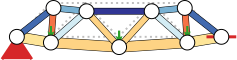
\includegraphics[width=0.8\linewidth]{../../Tooling/Icons/project}}}{}
	\IfStrEq{\theassignment}{Essay}
		{\def\theassignmenticon{\includegraphics[height=15em]{../../Tooling/Icons/essay}}}{}
	\IfStrEq{\theassignment}{Topic}
		{\def\theassignmenticon{
\includegraphics[height=15em]{../../Tooling/Icons/topic}}}{}
	\IfStrEq{\theassignment}{Inquiry}
		{\def\theassignmenticon{\includegraphics[height=15em]{../../Tooling/Icons/inquiry}}}{}
	\IfStrEq{\theassignment}{Homework}
		{\def\theassignmenticon{
\includegraphics[height=15em]{../../Tooling/Icons/homework}}}{}
	\IfStrEq{\theassignment}{Simulation}
		{\def\theassignmenticon{
\includegraphics[height=15em]{../../Tooling/Icons/simulation}}}{}
	\IfStrEq{\theassignment}{Method}
		{\def\theassignmenticon{\includegraphics[height=15em]{../../Tooling/Icons/method}}}{}
	\IfStrEq{\theassignment}{Experiment}
		{\def\theassignmenticon{\includegraphics[height=15em]{../../Tooling/Icons/experiment}}}{}
	\IfStrEq{\theassignment}{Lab}
		{\def\theassignmenticon{
\includegraphics[height=15em]{../../Tooling/Icons/lab}}}{}
	\IfStrEq{\theassignment}{Solutions}
		{\def\theassignmenticon{
\includegraphics[height=15em]{../../Tooling/Icons/solutions}}}{}
	\IfStrEq{\theassignment}{Describe}
		{\def\theassignmenticon{
\includegraphics[height=15em]{../../Tooling/Icons/describe}}}{}
	\IfStrEq{\theassignment}{Notes}
		{
			\def\theassignmenticon{
\includegraphics[height=15em]{../../Tooling/Icons/notes}}
			\def\nocontents{TRUE}
		}{}
	\IfStrEq{\theassignment}{Invoice}
		{
			\def\theassignmenticon{
\includegraphics[height=4em]{../../Tooling/Icons/invoice}}
			\def\nocontents{TRUE}
			\def\justonepage{TRUE}
		}{}
	\IfStrEq{\theassignment}{Exam}
		{
			\def\theassignmenticon{
				\includegraphics[height=15em]{../../Tooling/Icons/Exam}
				\vfill{}
				\vfill{}
				\begin{tabularx}{1\linewidth}{r>{\centering\arraybackslash}X}
				{\Large\textsf{\textbf{Name:}}} & \tabularnewline
				\cline{2-2}
				\tabularnewline
				\tabularnewline
				{\Large\textsf{\textbf{Date:}}} & \tabularnewline
				\cline{2-2}
				\tabularnewline
				\tabularnewline
				{\Large\textsf{\textbf{Time:}}} & \tabularnewline
				\cline{2-2}
				\tabularnewline
				\tabularnewline
				{\Large\textsf{\textbf{Location:}}} & \tabularnewline
				\cline{2-2}
				\end{tabularx}
			}
			\def\nocontents{TRUE}
		}{}
	
	\@ifundefined{theassignment}{
		\vfill{}
	}{
		\vspace{0.25in}
		\begin{center}
			\theassignmenticon
		\end{center}
		\vfill{}
	}
	\ifthenelse{\equal{\nocontents}{FALSE}}{\tableofcontents{}}{}
	\ifthenelse{\equal{\justonepage}{FALSE}}{\restoregeometry\pagebreak{}}{}
}

% Command reference
% \titleformat{⟨command ⟩}[⟨shape⟩]{⟨format⟩}{⟨label⟩}{⟨sep⟩}{⟨before-code⟩}[⟨after-code⟩]
% \titlespacing*{⟨command ⟩}{⟨left⟩}{⟨before-sep⟩}{⟨after-sep⟩}[⟨right-sep⟩]

% Format numbered headings
\titleformat{\section}[block]{}{}{0ex}
	{\tcbstartrecording\begin{CMESectionHeader}[\thesection]}[\end{CMESectionHeader}]
\titleformat{\subsection}[block]{}{}{0ex}
	{\begin{CMESubsectionHeader}[\thesubsection]}[\end{CMESubsectionHeader}]
\titleformat{\subsubsection}[block]{}{}{0ex}
	{\begin{CMESubsubsectionHeader}[\thesubsubsection]}[\end{CMESubsubsectionHeader}]

% Format numberless headings
\titleformat{name=\section,numberless}[block]{\sffamily\LARGE\bfseries\color{C0d}}{}{0ex}{}[]
\titleformat{name=\subsection,numberless}[block]{\sffamily\large\itshape\bfseries\color{C0d}}{}{0ex}{}[]
\titleformat{name=\subsubsection,numberless}[block]{\sffamily\normalsize\bfseries\color{C0d}}{}{0ex}{}[]

% Set heading spacings
\titlespacing*{\section}{0ex}{-1ex plus 1ex minus 1ex}{1ex plus 0ex minus 1ex}
\titlespacing*{\subsection}{0ex}{-1ex plus 1ex minus 1ex}{1ex plus 0ex minus 1ex}
\titlespacing*{\subsubsection}{0ex}{-1ex plus 1ex minus 1ex}{1ex plus 0ex minus 1ex}
